% \iffalse
\let\negmedspace\undefined
\let\negthickspace\undefined
\documentclass[journal,12pt,twocolumn]{IEEEtran}
\usepackage{cite}
\usepackage{amsmath,amssymb,amsfonts,amsthm}
\usepackage{algorithmic}
\usepackage{graphicx}
\usepackage{textcomp}
\usepackage{xcolor}
\usepackage{txfonts}
\usepackage{listings}
\usepackage{enumitem}
\usepackage{mathtools}
\usepackage{gensymb}
\usepackage{comment}
\usepackage[breaklinks=true]{hyperref}
\usepackage{tkz-euclide} 
\usepackage{listings}
\usepackage{gvv}                                        
\def\inputGnumericTable{}                                 
\usepackage[latin1]{inputenc}                                
\usepackage{color}                                            
\usepackage{array}                                            
\usepackage{longtable}                                       
\usepackage{calc}                                             
\usepackage{multirow}                                         
\usepackage{hhline}                                           
\usepackage{ifthen}                                           
\usepackage{lscape}
\usepackage[center]{caption} % center the captions to figure

\newtheorem{theorem}{Theorem}[section]
\newtheorem{problem}{Problem}
\newtheorem{proposition}{Proposition}[section]
\newtheorem{lemma}{Lemma}[section]
\newtheorem{corollary}[theorem]{Corollary}
\newtheorem{example}{Example}[section]
\newtheorem{definition}[problem]{Definition}
\newcommand{\BEQA}{\begin{eqnarray}}
\newcommand{\EEQA}{\end{eqnarray}}
\newcommand{\define}{\stackrel{\triangle}{=}}
\theoremstyle{remark}
\newtheorem{rem}{Remark}
\begin{document}

\newcolumntype{M}[1]{>{\centering\arraybackslash}m{#1}}
\newcolumntype{N}{@{}m{0pt}@{}}

\bibliographystyle{IEEEtran}
\vspace{3cm}

\title{NCERT 11.9.5} % TODO: change wrong problem number
\author{ee23btech11223 - Soham Prabhakar More% <-this % stops a space
}
\maketitle
\newpage
\bigskip

\renewcommand{\thefigure}{\theenumi}
\renewcommand{\thetable}{\theenumi}

\bibliographystyle{IEEEtran}

\textbf{Question:}\\
Which term of the following sequences:\\
(a) 2,$2\sqrt{2}$,4\dots is 128
\quad(b) $\sqrt{3}$,3,$3\sqrt{3}$\dots is 729\\
(c) $\frac{1}{3}$,$\frac{1}{9}$,$\frac{1}{27}$\dots is $\frac{1}{19683}$

\textbf{Answer:} (a) Let $x_1\brak{0} = 2$, $x_1\brak{1} = 2\sqrt{2}$, $x_1\brak{2} = 4$.
Since, $\frac{x_1\brak{1}}{x_1\brak{0}} = \frac{x_1\brak{2}}{x_1\brak{1}}$, the sequence $x_1\brak{n}$ is a G.P Series.
Let $r_1 = \frac{x_1\brak{1}}{x_1\brak{1}} = \sqrt{2}$, then the general term is $x_1\brak{n} = x_1\brak{0} r^{n-1}$.\\
Assume $n^{th}$ term is 128, which gives: 
\begin{align}
    x_1\brak{n} &= x_1\brak{0} r^{n-1} = 128\\
    \implies r_1^{n-1} &= \frac{128}{x_1\brak{0}}\\
    \implies n - 1 &= \log_{r_1}{\frac{128}{x_1\brak{0}}}
\end{align}
Using values from \tabref{Table:1}, 
\begin{align}
    \implies n - 1 &= \log_{\sqrt{2}}{\frac{128}{2}}\\
    \implies n - 1 &= \log_{\sqrt{2}}{64}\\
    \implies n - 1 &= \log_{\sqrt{2}}{\sqrt{2}^{12}}\\
    \implies n - 1 &= 12\\
    \therefore n &= 13
\end{align}
Thus the $13^{th}$ term of the G.P $x_1\brak{n}$ is 128.\\ 
\begin{align} x_1\brak{n} = x_1(0)r^{n}u[n] \end{align} where $u[0] = 1$.
\begin{figure}[h!]
    \centering
    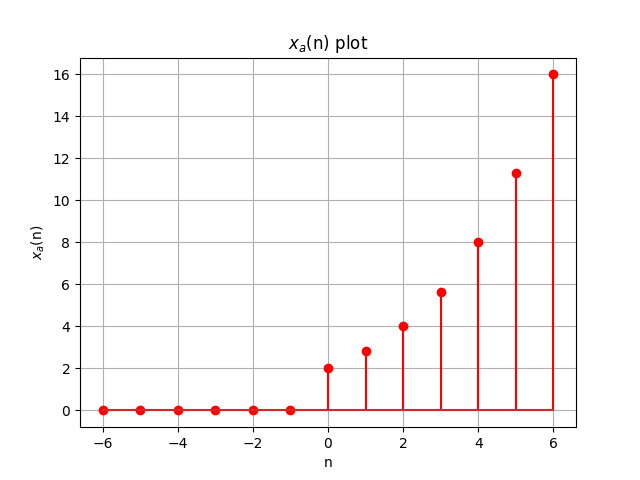
\includegraphics[width=0.5\textwidth]{figs/a.png}
    Fig. 1: Plot of $x_1$\brak{n} from n = -6 to 6
    \label{fig:img1}
\end{figure}
Taking the Z - transform:
\begin{align}
    X\brak{z} &= \sum_{n = -\infty}^{\infty}{x\brak{n} \cdot z^{-n}}\\
    \implies X\brak{z} &= \sum_{n = 0}^{\infty}{x\brak{0}r^{n}z^{-n}}\\
    \implies X\brak{z} &= x\brak{0}\sum_{n = 0}^{\infty}{r^n z^{-n}}\\
    \implies X\brak{z} &= \frac{x\brak{0}}{r}(\frac{1}{1 - \frac{r}{z}})\\
    \therefore X\brak{z} &= \frac{x\brak{0}z}{r(z - r)} \forall {\abs{z} > \abs{r}} \label{zresult}
\end{align}
\begin{align}
    \therefore X_1\brak{z} = \frac{\sqrt{2}z}{z - \sqrt{2}}\forall {\abs{z} > \sqrt{2}}
\end{align}
with ROC: \[ \abs{z} > \sqrt{2} \]

(b) Let $x_2\brak{0} = \sqrt{3}$, $x_2\brak{1} = 3$, $x_2\brak{2} = 3\sqrt{3}$.\\
Since $\frac{x_2\brak{1}}{x_2\brak{0}} = \frac{x_2\brak{2}}{x_2\brak{1}}$, the sequence $x_2\brak{n}$ is a G.P Series.
Let $r_2 = \frac{x_2\brak{1}}{x_2\brak{1}} = \sqrt{3}$, then the general term is $x_2\brak{n} = x_2\brak{0} r^{n-1}$.\\
Assume $n^{th}$ term is 729, which gives: 
\begin{align}
    x_2\brak{n} &= x_2\brak{0} r^{n-1} = 729\\
    \implies r_2^{n-1} &= \frac{729}{x_2\brak{0}}\\
    \implies n - 1 &= \log_{r_2}{\frac{729}{x_2\brak{0}}}
\end{align}
Using values from \tabref{Table:1},
\begin{align}
    \implies n - 1 &= \log_{\sqrt{3}}{\frac{729}{\sqrt{3}}}\\
    \implies n - 1 &= \log_{\sqrt{3}}{\frac{3^6}{\sqrt{3}}}\\
    \implies n - 1 &= \log_{\sqrt{3}}{\sqrt{3}^{11}}\\
    \implies n - 1 &= 11\\
    \therefore n &= 12
\end{align}
Thus the $12^{th}$ term of the G.P $x_2\brak{n}$ is 729.
\begin{align}  x_2\brak{n} = x_2(0)r_2^nu[n]  \end{align}
By \ref{zresult}, the Z-transform of $x_b$\brak{n}:
\begin{align} X_2\brak{z} = \frac{z}{z - \sqrt{3}} \end{align}
with ROC: \[ \abs{z} > \sqrt{3} \]
\begin{figure}[h!]
    \centering
    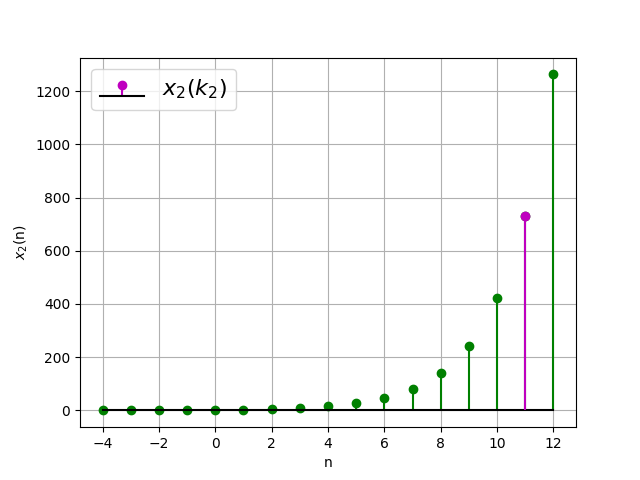
\includegraphics[width=0.5\textwidth]{figs/b.png}
    Fig. 2: Plot of $x_b$\brak{n} from n = -6 to 6
    \label{fig:img2}
\end{figure}

(c) Let $x_3\brak{0} = \frac{1}{3}, x_3\brak{1} = \frac{1}{9}, x_3\brak{2} = \frac{1}{27}$.\\
Since $\frac{x_3\brak{1}}{x_3\brak{0}} = \frac{x_3\brak{2}}{x_3\brak{1}}$, the sequence $x_3\brak{n}$ is a G.P Series.
Let $r_3 = \frac{x_3\brak{1}}{x_3\brak{1}} = \frac{1}{3}$, then the general term is $x_3\brak{n} = x_3\brak{0} r^{n-1}$.\\
Assume $n^{th}$ term is $\frac{1}{19683}$, which gives: 
\begin{align}
    x_3\brak{n} &= x_3\brak{0} r_3^{n-1} = \frac{1}{19683}\\
    \implies r_3^{n-1} &= \frac{1}{19683 x_3\brak{0}}\\
    \implies n - 1 &= \log_{r_3}{\frac{1}{19683 x_3\brak{0}}}
\end{align}
Using values from \tabref{Table:1},
\begin{align}
    \implies n - 1 &= \log_{\frac{1}{3}}{\frac{1}{19683 \frac{1}{3}}}\\
    \implies n - 1 &= \log_{\frac{1}{3}}{\frac{1}{6561}}\\
    \implies n - 1 &= \log_{\frac{1}{3}}{3^{-8}}\\
    \implies n - 1 &= 8\\
    \therefore n &= 9
\end{align}
Thus the $9^{th}$ term of the G.P $x_3\brak{n}$ is $\frac{1}{19683}$.
\begin{align}  x_3\brak{n} = x_3(0)r_3^{n}u[n]  \end{align}
By \ref{zresult}, the Z-transform of $x_3\brak{n}$:
\begin{align}
    X_3\brak{z} = \frac{z}{z - \frac{1}{3}}
    \implies X_3\brak{z} = \frac{3z}{3z - 1}
\end{align} with ROC: \[ \abs{z} > \frac{1}{3} \]

\begin{figure}[h!]
    \centering
    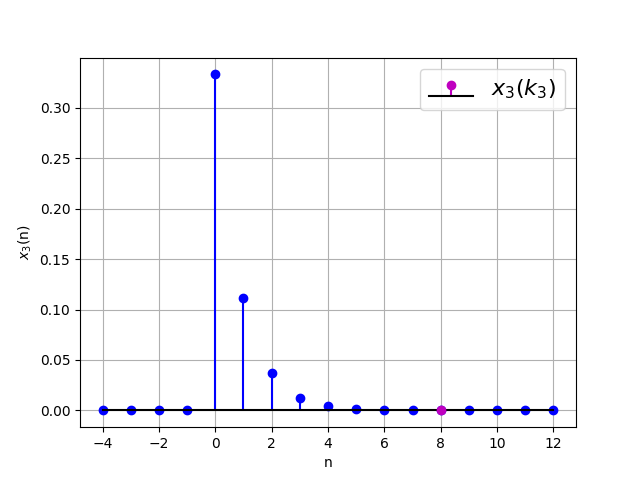
\includegraphics[width=0.5\textwidth]{figs/c.png}
    Fig. 3: Plot of $x_3$\brak{n} from n = -6 to 6
    \label{fig:img3}
\end{figure}

\begin{table}[ht]
    \begin{tabular}{ | >{\centering\arraybackslash}m{2cm} | >{\centering\arraybackslash}m{3cm} | >{\centering\arraybackslash}m{2cm} | @{}m{0pt}@{} }
    \hline
    \textbf{Parameter} & \textbf{Explaination} & \textbf{Values} &\\[10pt]
    \hline
    r & Common ratio of G.P & $\frac{1}{3}$ &\\[10pt]
    \hline
    $c_n$ & Sequence & $\frac{1}{3}$,$\frac{1}{9}$,$\frac{1}{27}$\dots &\\[10pt]
    \hline
    $x_c(n)$ & Function equivalent of sequence $c_n$ & --- &\\[10pt]
    \hline 
    $X_c(n)$ & Z-transform of $c_n$ & --- &\\[10pt]
    \hline 
    \end{tabular}
    \begin{center}
        \text{Table 3: Variables used in (c)}
    \end{center}
\end{table}


\end{document}

